\chapter{Background}
\begin{chapquote}{Isaac Asimov, \textit{The Secrets of the Universe}}
The job of science will never be done, it will just sink deeper and deeper into never-ending complexity.
\end{chapquote}

In this chapter, we give an overview of the related technologies and prior works that are important to this thesis.  These projects and ideas are the building blocks of the FPsPIN prototype system.

\section{SmartNIC architectures}
SmartNICs from different vendors tend to have different architectures, but they can be classified by the \emph{datapath design} largely into two categories: \emph{on-path} versus \emph{off-path}~\cite{liu_offloading_2019, wei_characterizing_2023}.  We show a brief overview of both paradigms in \Cref{fig:smartnic-datapaths}.  In addition to data path designs, there is also an increasing trend to use \emph{reconfigurable hardware} to implement SmartNICs.  We introduce the various paradigms and discuss how most commodity SmartNICs fit into these categories.

\begin{figure}[tp]
    % https://tex.stackexchange.com/a/218414/150873
    % preliminary
    \sbox\twosubbox{%
      \resizebox{\dimexpr0.95\textwidth-1em}{!}{%
        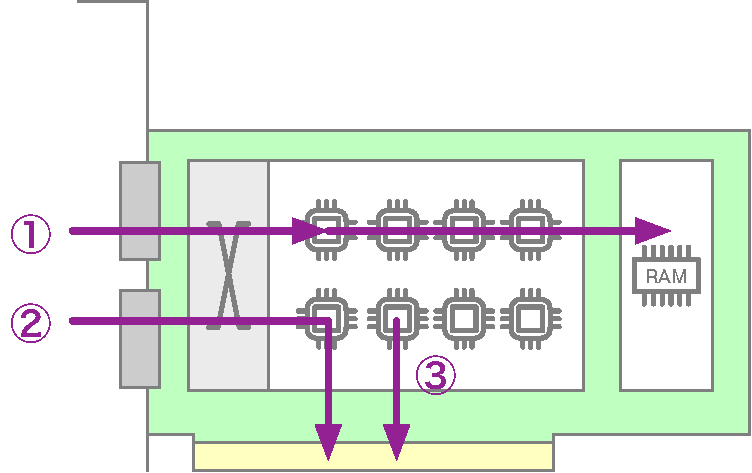
\includegraphics[height=3cm]{thesis/figures/on-path-smartnics.pdf}%
        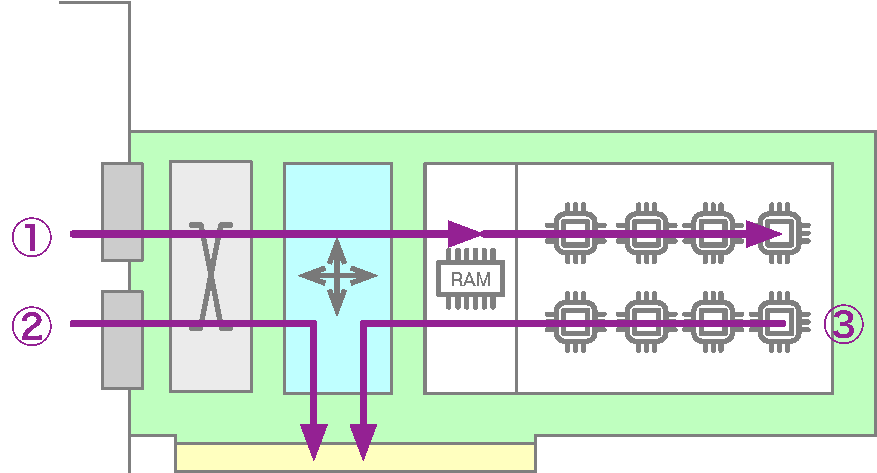
\includegraphics[height=3cm]{thesis/figures/off-path-smartnics.pdf}%
      }%
    }
    \setlength{\twosubht}{\ht\twosubbox}
    
    \centering
    
    \subcaptionbox{On-path SmartNICs.  \label{fig:on-path-smartnic}}{%
      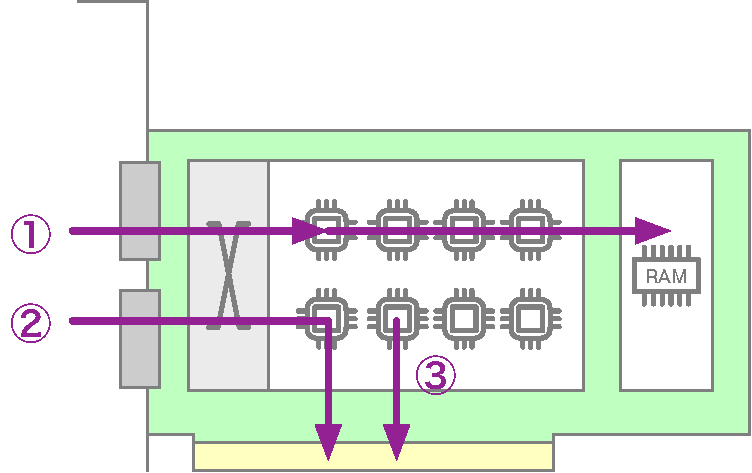
\includegraphics[height=\twosubht]{thesis/figures/on-path-smartnics.pdf}%
    }\quad
    \subcaptionbox{Off-path SmartNICs.  The PCIe switch is marked in blue.  \label{fig:off-path-smartnic}}{%
      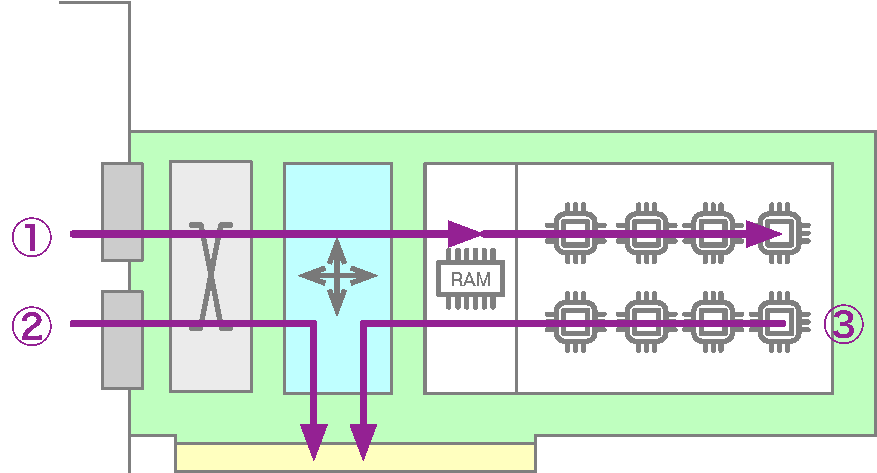
\includegraphics[height=\twosubht]{thesis/figures/off-path-smartnics.pdf}%
    }
    \caption[Overview of different SmartNIC data path designs]{Overview of different PCIe-based SmartNIC data path designs.  The purple arrows denote different data flow interactions between the NIC cores and the host CPU upon incoming traffic.  \circled{1}: offloaded traffic; \circled{2}: (non-offloaded) host traffic; \circled{3}: host-NIC interactions.} \label{fig:smartnic-datapaths}
\end{figure}

\paragraph{On-path SmartNICs} \emph{On-path} SmartNICs, also known as \emph{bump-in-the-wire}, have the \emph{processing elements} (PE) sit on the packet processing path and have the ability to modify incoming and outgoing packets.  \Cref{fig:on-path-smartnic} demonstrates the flow of packet data on these SmartNICs: incoming packets gets assigned to NIC PEs and either gets processed on the NIC as offloaded traffic (\circled{1}), or steered to the host (\circled{2}).  The NIC PEs can further interact with the host CPU over the PCIe interface (\circled{3}).  Examples of on-path SmartNICs include the Marvell LiquidIO~\cite{noauthor_marvell_nodate}, Netronome Agilio CX~\cite{noauthor_agilio_nodate}, as well as research systems~\cite{guo_framework_2022, wang_fpganic_2022}.

The most important benefit in this design is that the SmartNIC PEs have very low latency access to packet data (\circled{1}), allowing efficient NIC-only transactions (that do not involve the host).  Downsides of this design mainly come from the fact that regular, non-offloaded host traffic still require SmartNIC PEs to steer to the host (\circled{2}).  This results in degraded host traffic performance when the NIC is heavily loaded~\cite{liu_offloading_2019}.  Another difficulty is due to the low-latency requirement from the on-path nature of the SmartNIC data path, forcing a low-level interface that is difficult to program against.

\paragraph{Off-path SmartNICs} In contrary to on-path SmartNICs, \emph{off-path} SmartNICs have the packet PEs, usually as a separate \emph{system-on-chip} (SoC) \emph{off} the regular packet data path.  We show the flow of packet data on these SmartNICs in \Cref{fig:off-path-smartnic}: compared to the on-path paradigm, an extra PCIe switch allows both the host CPU and the packet PEs to act as fully-capable \emph{hosts} to the NIC.  The switch steers the incoming packets from the network fabrics to the NIC PEs (\circled{1}) or the host (\circled{2}), according to configurable rules.  An example of this SmartNIC design is the NVIDIA BlueField~\cite{nvidia_corporation_nvidia_2021}.

Thanks to the packet processor not being on the critical path to the host, the off-path paradigm allows for more complicated software stacks on the SmartNIC.  This allows for a full network stack and operating system, usually the Linux kernel, on the SmartNIC cores, as well as more user-friendly programming interfaces.  However, the addition of the PCIe switch significantly increases the latency of NIC-offloaded tasks (\circled{1}) and NIC-host interactions (\circled{3}) compared to on-path designs~\cite{wei_characterizing_2023}.

\paragraph{Reconfigurable hardware} While most commercial vendors implement the SmartNIC PEs as fixed-purpose SoCs with special accelerators, there are increasing attention into building \emph{Field-Programmable Gate Array} (FPGA) into the SmartNIC.  This results in architectures that are either SoCs coupled with an FPGA or entirely FPGA-centric designs.  Examples include in-house deployments inside Microsoft Azure~\cite{firestone_azure_2018}, products from Intel~\cite{intel_intel_nodate} and AMD~\cite{xilinx_alveo_2020, xilinx_alveo_2022}, as well as research systems~\cite{wang_fpganic_2022, khazraee_rosebud_2023}.

FPGA-enabled SmartNICs excel in reconfigurability.  While having purpose-built SoCs coupled with a pre-determined set of accelerators can provide the highest-possible performance, they cannot evolve to accommodate the changing demands of the workload.  Reconfigurable solutions allow users to customise the SmartNIC hardware \emph{after} the hardware is built by implementing new, custom accelerators in the FPGA.  This offers the customers great flexibility and more possibilities for accelerated offloading.  They are also suitable in domains with a small volume to the point where it is not cost effective to tape out a custom \emph{application-specific integrated circuit} (ASIC) with domain-specific accelerators, such as in telecommunications and research.

\section{sPIN} \label{sec:background-spin}

\begin{figure}[tp]
    \centering
    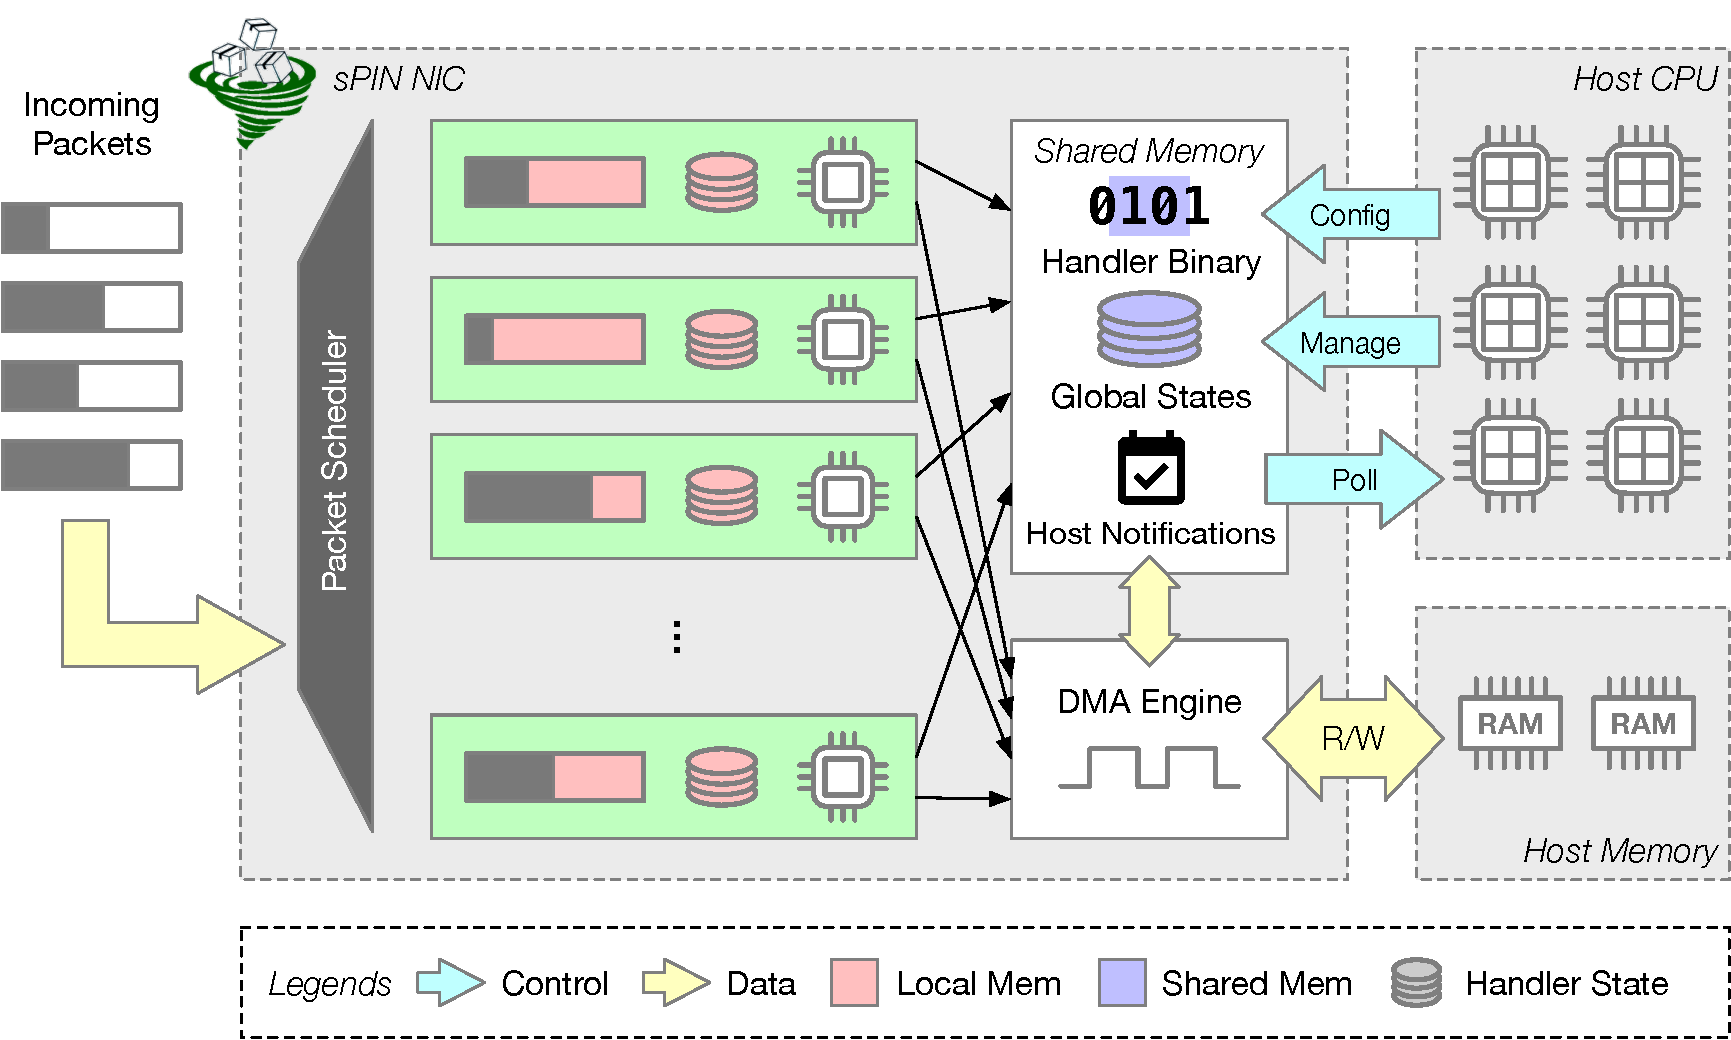
\includegraphics[width=.9\textwidth]{thesis/figures/spin-arch.pdf}
    \caption{Overview of the sPIN architecture.}
    \label{fig:spin-arch}
\end{figure}

\begin{figure}[tp]
    \centering
    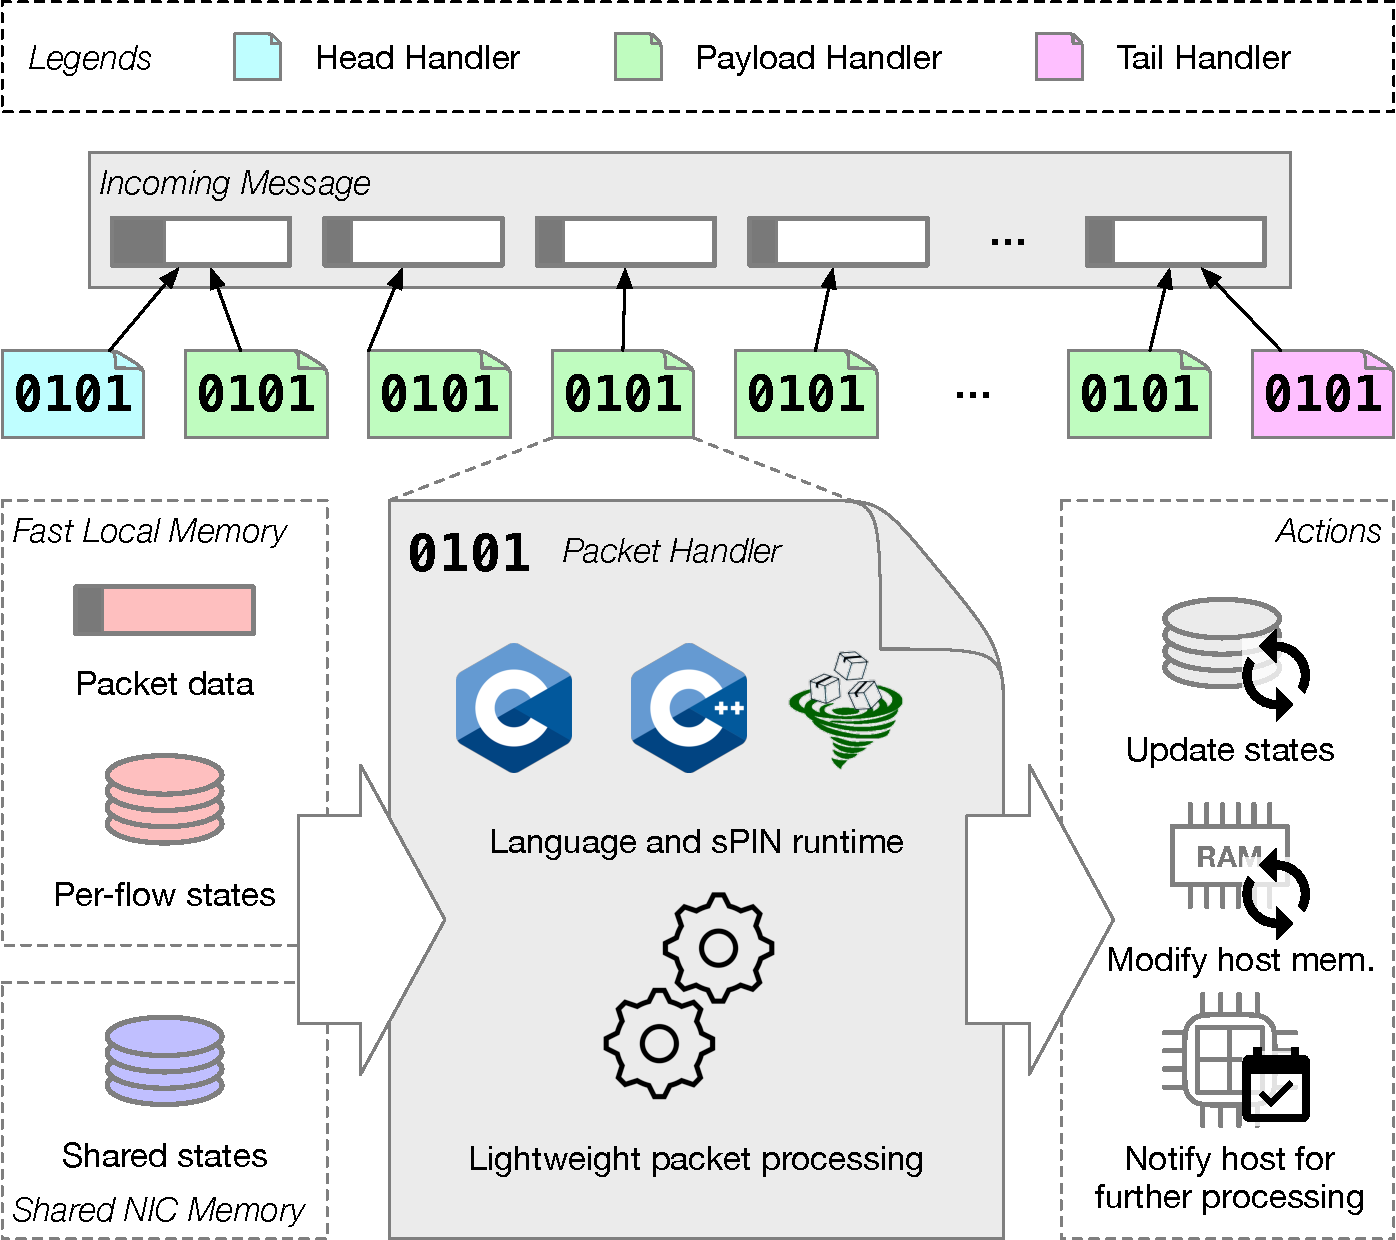
\includegraphics[width=.8\textwidth]{thesis/figures/spin-handlers.pdf}
    \caption{Consumption of packets of an incoming message by packet handlers.  Inputs and actions of individual handlers are shown in the zoom-in view.} \label{fig:spin-handlers}
\end{figure}

\emph{streaming Processing in the Network} (sPIN)~\cite{hoefler_spin_2017} is a portable programming model that allows a programmer to offload simple packet processing functions of a networked application code the NIC.  sPIN is designed to exploit packet-level parallelism through execution of short, lightweight \textit{packet handlers}.  The \emph{streaming} semantics of sPIN comes from its \emph{flow-oriented} nature in keeping a state for each traffic flow\footnote{We use \emph{flow} and \emph{message} interchangeably in the context of sPIN in this thesis.} (e.g.\ TCP/UDP connections, MPI messages, etc.).  This allows for efficient packet processing with higher expressiveness in comparison to other offloaded packet processing models, such as Portals~4~\cite{bosshart_p4_2014} or eBPF/XDP~\cite{vieira_fast_2021}, in which packet processing functions are stateless.  An overview of the sPIN architecture is shown in \Cref{fig:spin-arch}.

\emph{Packet handlers} and how they behave is the core of sPIN: the possible actions from the handlers together with the packet scheduling requirements define sPIN as a \emph{network instruction set architecture} (NISA)~\cite{hoefler_spin_2017}.  We visualise how sPIN handlers process packet data in \Cref{fig:spin-handlers}.  Handlers take the packet data and per-flow state as input and perform one or many of the following actions: \emph{update the flow state}, \emph{read from and write to host memory}, and \emph{notify the host for further action}.  On incoming packets of a flow, the programming model further defines three types of handlers for execution on the packet PEs:

\begin{itemize}
    \item A \emph{head} handler to be executed on the first packet of a flow; this is guaranteed to be the first handler executed for a given flow.
    \item A \emph{payload} handler to be executed on every packet; they are guaranteed to be scheduled only after the \emph{head} handler finishes execution.
    \item A \emph{tail} handler to be executed on the last packet of the flow; this is guaranteed to be scheduled only after all \emph{payload} handlers finish execution.
\end{itemize}

Packet handlers are scheduled and executed concurrently on the SmartNIC PEs, namely \emph{handler processing units} (HPU).  A \emph{packet scheduler} schedules incoming packets on the HPUs for execution w.r.t.\ the handler scheduling dependency requirements.  The HPUs access packet data and per-flow states in fast local memory and shared states in the shared NIC memory.  They access host memory through a device-level DMA engine between the host and shared NIC memory.  The host CPU functions as the control plane and is in charge of programming the scheduler and the HPUs, host and NIC memory allocation and initialisation, as well as processing host notifications from the HPUs.

\section{FPGA and design reuse} \label{sec:fpga-basics}

\emph{Field-programmable gate arrays} (FPGA)~\cite{brown_field-programmable_1992} is a type of integrated circuit that allows runtime \emph{reconfiguration} after being manufactured.  They consist of an array of \emph{configurable logic blocks} (CLB) that can function either as \emph{lookup tables} (LUT) or \emph{flip-flops} (FF), and programmable routing resources that connect the input and output of CLBs.  LUTs are used to implement combinational logic and FFs sequential logic.  A \emph{bitstream} for an FPGA, when flashed onto the device, configures all CLBs and routing resources into a specific digital logic design.  FPGAs can be used to validate hardware designs before they are taped out into ASICs since large designs take way too long to simulate and bring up complicated software.  They are also used for situations that call for reconfigurability, such as building custom accelerators in the cloud, as well as for products with a small volume where producing ASIC is cost-inefficient.

\paragraph{Design reuse} To facilitate development of new microchips, hardware \emph{intellectual property} (IP) vendors package their hardware function blocks as \emph{IP blocks} and redistribute them to customers for integration into their design.  For interoperability with other IP vendors as well as customer designs, IP blocks adopt industrial standards for \emph{bus protocols}.  On the other hand, if design components do not speak the same bus protocol, an \emph{adapter} is needed.  Adapters consume hardware resources and may impact performance depending on the complexity of the protocol; a perfect adapter may not even be possible in case of mismatch of semantics between the protocols.

The simplest bus protocol for signaling the validity and acknowledgement of data is the \emph{ready-valid} protocol.  It consists of two extra wires in addition to the data signals: \emph{ready} denotes that the receiver can accept data, and \emph{valid} denotes that the data driven by the sender is valid.  A \emph{beat} of data is successfully transmitted if both ready and valid are held high for one clock cycle; the receiver can assert \emph{back pressure} by de-asserting the ready signal.  A common variant of the protocol is a \emph{valid} protocol, where the ready signal is missing and implied to be always high.  This indicates that the sender has no internal buffer for dealing with possible back pressure from the receiver and that the receiver always has to be ready for data.  If the receiver could not keep up with the data rate on the bus, a valid beat of data would be dropped.

The \emph{Advanced eXtensible Interface} (AXI)~\cite{arm_limited_amba_2003, arm_limited_amba_2010} is a family of \emph{on-chip} communication bus protocols designed to connect IP blocks in a hardware design.  AXI protocols follow a \emph{master-slave} design where the bus master initiates transactions and the bus slave responds.  The protocol has three flavours, designed for different use cases.  \emph{AXI-MM} is designed for high-performance memory-mapped read and write access from processor-like masters on addressable memory-like slaves.  \emph{AXI-Lite} is designed for light-weight memory-mapped access for lower performance situations; it does not support advanced features like bursting, narrow transfers or interleaved requests, making it a lot simpler to implement.  \emph{AXI-Stream} is designed for streaming data from master to slave without addressing semantics.

\paragraph{Hardware used in this thesis} We use the VCU1525 Development Kit from Xilinx\footnote{\url{https://www.xilinx.com/products/boards-and-kits/vcu1525-a.html}} for development and testing of FPsPIN.  The board comes with a Xilinx UltraScale+ VU9P FPGA, 64 GB of DDR4 memory and 16 lanes of PCIe 3.0.  In addition, it also has 2 QSFP+ cages that support up to 100 Gbps Ethernet; each QSFP+ port can be split into 4 25 Gbps Ethernet ports with a breakout cable\footnote{\url{https://www.fs.com/de-en/products/70537.html}}.  As later to be introduced in \Cref{chap:hardware} and \Cref{chap:eval}, we operate the 100 Gbps Ethernet ports using a loopback cable without splitting them.

\section{PsPIN and RISC-V} \label{sec:background-pspin}

\begin{figure}[tp]
    \centering
    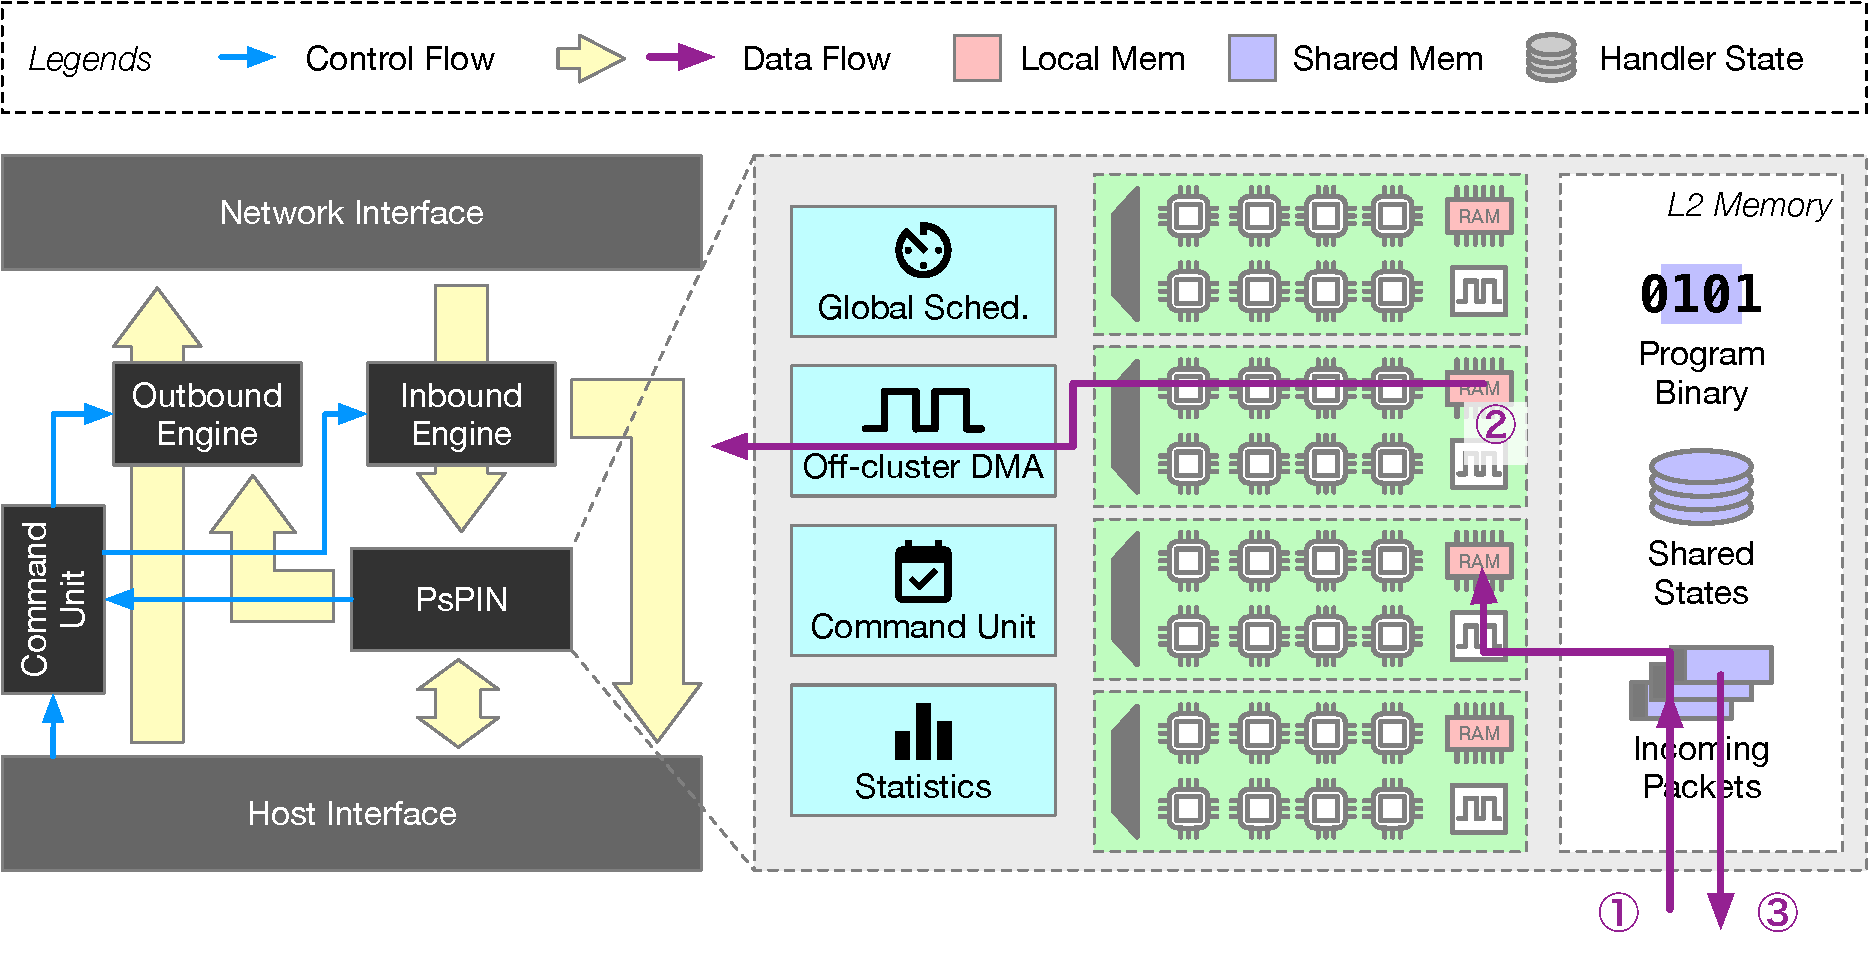
\includegraphics[width=\textwidth]{thesis/figures/pspin-arch.pdf}
    \caption{Overview of the PsPIN architecture and NIC model.  The purple arrows denote the three major data flows cross-referenced in \Cref{sec:background-pspin}.} \label{fig:pspin-arch}
\end{figure}

While sPIN defines the streaming in-network-computing NISA, it does not specify the exact micro-architecture of sPIN-enabled NICs such as the ISA for the HPUs or the exact memory hierarchy on the NIC.  PsPIN~\cite{di_girolamo_pspin_2021} is the reference ASIC implementation of sPIN, ready to be integrated into the packet data path of existing NIC designs.  It specifies the interface of a NIC of which PsPIN can be integrated into.  PsPIN uses the CPU cores developed by the PULP~\cite{rossi_pulp_2015} project to implement the HPUs.  It groups the HPU cores into \emph{clusters} for a hierarchical memory architecture and multi-level scheduling.  An overview of the PsPIN architecture and NIC model is shown in \Cref{fig:pspin-arch}.

The control flow of PsPIN starts with new packets arriving from the NIC.  The NIC inbound engine generates a \emph{handler execution request} (HER) that contains metadata for scheduling the packet on a HPU, including the address of packet data in the NIC memory and the address of the sPIN handler functions.  The \emph{global} scheduler then resolves the scheduling dependencies according to the sPIN NISA as described in \Cref{sec:background-spin} and forwards individual \emph{tasks} to the \emph{cluster} schedulers.  The cluster scheduler forwards the incoming tasks to the HPUs local to that cluster for execution, and collects the finish notifications from the HPUs called \emph{feedbacks}.  It forwards the feedback through the global scheduler back to the NIC inbound engine, such that the packet buffer can be deallocated and reused.

Three major data flows cover the full cycle of packet processing in PsPIN, all of which are driven by various DMA engines, allowing fast data movement and latency hiding.  The inbound packet data from the NIC inbound engine to the \emph{L2} packet buffer is handled by the DMA engine in the NIC inbound engine; the data is further DMA'ed into the cluster-local \emph{L1} memory by the cluster DMA engine (\circled{1}).  Host memory access by the HPUs flow from L2 or L1 to the host memory and is handled by the \emph{off-cluster} DMA engine (\circled{2}).  Outgoing packet data from L2 or L1 is handled by the DMA engine inside the NIC outbound engine (\circled{3}).  PsPIN exposes AXI slave ports for access to the internal interconnect by the NIC DMA engines.

\emph{RISC-V}~\cite{asanovic_instruction_2014, waterman_risc-v_2019} is an open \emph{instruction set architecture} (ISA) developed at UC Berkeley and now hosted by the non-profit RISC-V Foundation.  It has much momentum in the community of both research groups and companies due to its free and open nature and has seen many open-source~\cite{zhao_sonicboom_2020, asanovic_rocket_2016, rossi_pulp_2015} and commercial~\cite{t-head_t-head_nodate,sifive_sifive_2022} implementations.  The openness of RISC-V to custom extensions and the abundance of open-source implementation facilitate diverse architecture research~\cite{lee_keystone_2020, shao_simba_2019, genc_gemmini_2019, lin_panic_2020, khazraee_rosebud_2023} where it was previously almost impossible to build hardware prototypes due to the closed and proprietary nature of existing ISAs and expensive and restrictive licensing of processor IPs.

\section{Corundum} \label{sec:background-corundum}

Corundum~\cite{forencich_corundum_2020} is an open-source, FPGA-based NIC and a platform for in-network computing.  The project supports 10/25/100 Gbps Ethernet on Xilinx and Intel platforms.  It offers a high performance, custom PCIe DMA system and open-source platform-agnostic IPs including the Ethernet MAC and AXI infrastructure.  Corundum also has support for scatter/gather DMA, checksum offloading, as well as support for multi-interface multi-port operation.  It offers a full software stack on Linux, exposing fine-grained scheduling and queue management tunables to the user.  The comprehensive feature set and open code base makes Corundum an ideal platform for high-performance network research.

The most important design of Corundum for the scope of this thesis is its support for custom hardware logic to extend the functionality of the NIC.  The code base allows developers to pack custom logic into a self-contained \emph{application block} with access to the control path, data path, and DMA subsystems.  Corundum's software stack also provides kernel interfaces for custom drivers and user space utilities, as well as example designs.  As a result, Corundum makes a perfect candidate platform for integrating a packet processing cluster like PsPIN to build a full SmartNIC.

\section*{Now that we have all the pieces\ldots}

We have now introduced the essential components towards building FPsPIN.  However, even though we have the major parts of the SmartNIC ready, we still need to integrate them to create a complete SmartNIC.  As we have shown in \Cref{fig:full-system}, apart from the PsPIN processing cluster marked in green, we also need the data path engines and PCIe interface in hardware.  Some of these components come from Corundum; others, such as the matching engine that determines which packets are going to be processed by the cluster, need to be designed and implemented from scratch.  In addition, as Corundum and PsPIN are developed independently, we need various bus interconnects to bridge the control and data paths.  We explain the design and implementation of these hardware components in \Cref{chap:hardware}.  The host-side device drivers and the runtime library for interfacing with the processing cluster needs to be implemented as well; we discuss this in detail in \Cref{chap:software}.  We present in \Cref{chap:spin-revisited} the shortcomings of the sPIN NISA that we discovered while building FPsPIN.  Finally, we explain in detail in \Cref{chap:eval} the experiments we conduct to showcase the functionality and performance of FPsPIN.  Let's dive in!